\section{Desarrollo}
%Deben explicarse los métodos numéricos que utilizaron y su aplicación al problema
%concreto involucrado en el trabajo práctico. Se deben mencionar los pasos que si-
%guieron para implementar los algoritmos, las dificultades que fueron encontrando y la
%descripción de cómo las fueron resolviendo. Explicar también cómo fueron planteadas
%y realizadas las mediciones experimentales. Los ensayos fallidos, hipótesis y conjeturas
%equivocadas, experimentos y métodos malogrados deben figurar en esta sección, con
%una breve explicación de los motivos de estas fallas (en caso de ser conocidas).

\subsection{Matrices Banda}

\subsubsection{Por que queda una matriz Banda}
La obtención de la matriz Banda esta ligada directamente con nuestro sistema de ecuaciones, con la ecuación de calor discretizada y con el orden de numeración de las variables. \\
Por ejemplo, la siguiente figura  muestra un ejemplo de instancia de un parabrisa:

    \begin{figure}[H]
    \centering
    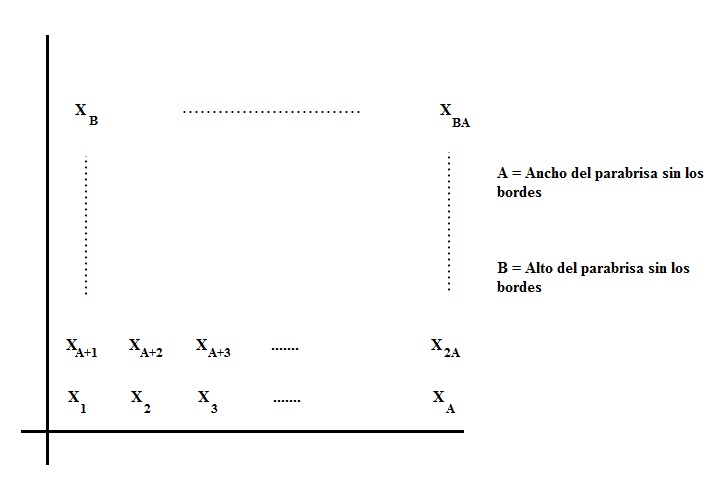
\includegraphics[scale=0.7]{graphs/mapa.jpg}\caption{Cada X$_i$ representa un punto de la discretizacin de este parabrisa}
      \end{figure}
      
      
      
Empezemos a despejar las variables y armar nuestro sistema de ecuaciones:\\
    \begin{itemize}
    \item  X$_1$ = (X$_2$ + X$_{a+1}$ - 100 - 100)/4\\
            4*X$_1$ - X$_2$ - X$_{a+1}$ = -200 
            
    \item X$_2$ = (X$_1$ + X$_{a+2}$ + X$_3$ - 100)/4\\
            4*X$_2$ - X$_1$ - X$_{a+2}$ - X$_3$ = -100 
    
    \end{itemize}
    
    Así, sucesivamente hasta despejar todas las incógnitas y completar el sistema. Como consecuencia del uso de la ecuación de calor, cada incógnita va a depender de una incógnita que este a la izquierda, derecha, arriba, y abajo de la misma. Esto se interpreta como que cada una de las variables, se relaciona con a lo sumo dos variable pegadas y con dos variable que están a A de distancia de la variable en estudio (Decimos a lo sumo, para especificar el caso de las variables que estás pegadas a los bordes, o sanguijuelas). Esto, y que empezamos despejando desde el extremo inferior izquierdo del parabrisa, son las causas de que la matriz quede establecida como una matriz banda.\\
    Armando la matriz asociada al sistema de ecuaciones, nos da como resultado la siguiente figura, que muestra la relación de las variables con la distancia A.
    
        \begin{figure}[H]
    \centering
    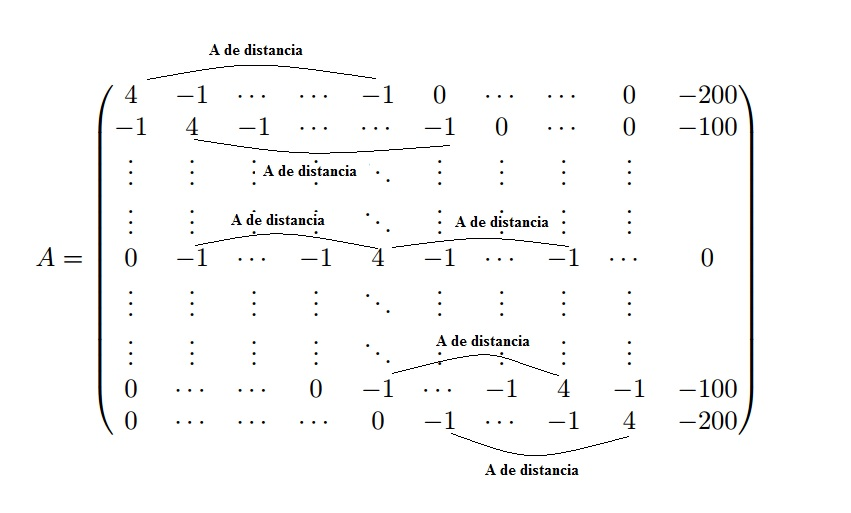
\includegraphics[scale=0.7]{graphs/matriz.jpg}}
      \end{figure}
    
    


\subsubsection{Eliminacion Gaussiana}
Algorítmicamente, la idea es similar a la Eliminacion Gaussiana clásica. En este caso, como consecuencia de nuestro sistema de ecuaciones, la matriz resultante del sistema asociado se compone por una diagonal integrada:
\begin{itemize}
\item Por números 4, si se trata de una posicion sin sanguijuela.
\item Por números 1, si se trata de una posición con sanguijuela.
\end{itemize}

Las demás posiciones de la matriz se llenan con 1, -1 o 0, depende el caso.\\ 
Aprovechando las características de la diagonal y los posibles números, no es necesario intercambiar filas debido a que, al triangular, la diagonal nunca va a tener números 0. Además, ya que estas matrices tienen la cualidad de tener diagonales de 0 en los extremos superior derecho e inferior izquierdo nos simplifica las siguiente operacion en relación al algoritmo clásico:

\begin{itemize}
\item No es necesario restar la fila completa, por la presencia de números 0 en el extremo superior derecho.
\item Por cada paso que avanzo en la diagonal, no es necesario realizar la resta de filas hasta abajo, por la presencia de 0 en el extremo inferior izquierdo  
\end{itemize}

Además, en el momento de ir consiguiendo los número 0 de la triangulación, se los asigna directamente para no tener problemas de precisión. Resumiendo, el codigo quedaría asi:\\
 \begin{algorithm}[H]
\caption{EliminacionGaussiana0()}
\begin{algorithmic}[1]

\For{$j = 0; j < filas; j++$}
    
    \For{$(i = j+1; (i <= j + ancho) && (i < filas); i++)}$}
    
        \State coeficiente = (Obtener(i,j)/Obtener(j,j));
		\State RestarFila0(coeficiente, j, i, j+1);
		
	\EndFor 
    \State cerosAIzquierda(j,j);
	
	\EndFor
	
\end{algorithmic}
\end{algorithm}
\textit{Siendo ancho, el ancho del parabrisa, es decir el ancho de la banda, filas la cantidad de filas de la matriz y restarFila0 es la función para restar filas con la particularidad de lo expresado anteriormente}
	
	

















\subsubsection{Factorización LU}

\subsubsection{BackWard Substitution}
Aprovechando la estructura de las matrices bandas, al aplicar Eliminación Gaussiana, la matriz triangular superior resultante hereda las bandas superiores de 0. Ante esto el algoritmo clásico de BackWard Substitution se puede modificar para aprovechando que algunos valores con 0. El caso de ForWard Substitution es análogo


\subsubsection{Eliminar sanguijuela}
Ante lo observado y desarrollado, se llevará a cabo una cierta cantidad de experimentaciones para poder contrastar las siguiente  hipótesis:\\

\begin{enumerate}
\item Al utilizar factorización LU y la formula de Sherman-Morrison, el algoritmo de EliminarSanguijuela logra una mejor performance en los casos de que existieran sanguijuelas unitarias.
\item Por otra parte quisimos ver que pasaba al modificar la granularidad. En otras palabras, verificar si al disminuir la misma, la posibilidad de encontrar sanguijuelas unitarias también disminuía, y en consecuencia el algoritmos modificado con Sherman-Morrison bajaba en su rendimiento, asemejándose en complejidad al algoritmo original\\
\end{enumerate}


Para verificar la hipótesis (1), se llevará a cabo una experimentación tomando 3 instancias, cada una describiendo el caso mejor, caso promedio y caso peor de la cantidad de sanguijuelas unitarias. Para concluir se tomarán los tiempos de ejecución del algoritmo original y el algoritmo modificado por Sherman-Morrison por cada instancia y se los comparará.\\
Para verificar la hipótesis (2), se llevará a cabo otra experimentación tomando 3 instancias exactamente iguales, a excepción de la granularidad, que se la irá cambiando.
